\documentclass[12pt, oneside, titlepage]{article}   	% use "amsart" instead of "article" for AMSLaTeX format

\usepackage{graphicx}
\graphicspath{ {\string} }
\usepackage{subcaption}

%%%%%%%%%%%%%%%%%%%%%%%%%%%%%%%%%%%%%%%%%%%%%%%%%%%%
% set up packages
%%%%%%%%%%%%%%%%%%%%%%%%%%%%%%%%%%%%%%%%%%%%%%%%%%%%
\usepackage{geometry}                
\usepackage{textcomp}                
\usepackage{amsmath}                
\usepackage{graphicx}                
\usepackage{amssymb}                
\usepackage{fancyhdr}                
\usepackage{subcaption}                
\usepackage{bm}                
\usepackage{tabularx}                

\usepackage{lineno}
% package for comments
\usepackage{soul}

\usepackage[breaklinks=true]{hyperref}

\usepackage[superscript,noadjust]{cite} % puts dash in citations to abbreviate
\usepackage [autostyle, english = american]{csquotes} % sets US-style quotes

\usepackage{etoolbox} % block quotes

\usepackage{float}
\usepackage{color}

\usepackage{pgf}
\usepackage{tikz}
\usepackage{eqnarray}

\usepackage{listings} % code blocks
\usepackage{setspace}

\usepackage{lscape}

% tikz background
\usetikzlibrary{backgrounds, fit}


\usepackage{natbib}
%\bibliographystyle{abbrvnat}
\setcitestyle{authoryear,open={(},close={)}}

%%%%%%%%%%%%%%%%%%%%%%%%%%%%%%%%%%%%%%%%%%%%%%%%%%%%
% call packages
%%%%%%%%%%%%%%%%%%%%%%%%%%%%%%%%%%%%%%%%%%%%%%%%%%%%	
\geometry{letterpaper, marginparwidth=60pt} % sets up geometry              		
\linenumbers % adds line numbers 
\MakeOuterQuote{"} % sets quote style
\doublespacing % setspace

%%%%%%%%%%%%%%%%%%%%%%%%%%%%%%%%%%%%%%%%%%%%%%%%%%%%
% patches with etoolbox 
%%%%%%%%%%%%%%%%%%%%%%%%%%%%%%%%%%%%%%%%%%%%%%%%%%%%	
% block quotes
\AtBeginEnvironment{quote}{\small}

% linenumbers
\makeatletter
\patchcmd{\@startsection}{\@ifstar}{\nolinenumbers\@ifstar}{}{}
\patchcmd{\@xsect}{\ignorespaces}{\linenumbers\ignorespaces}{}{}
\makeatother

%%%%%%%%%%%%%%%%%%%%%%%%%%%%%%%%%%%%%%%%%%%%%%%%%%%%
% tikzlibrary modifications
%%%%%%%%%%%%%%%%%%%%%%%%%%%%%%%%%%%%%%%%%%%%%%%%%%%%	
\usetikzlibrary{fit}
\usetikzlibrary{positioning}
\usetikzlibrary{arrows}
\usetikzlibrary{automata}

%%%%%%%%%%%%%%%%%%%%%%%%%%%%%%%%%%%%%%%%%%%%%%%%%%%%
% page formatting; exact 1 in margins
%%%%%%%%%%%%%%%%%%%%%%%%%%%%%%%%%%%%%%%%%%%%%%%%%%%%
\pagestyle{plain}                                                     

\setlength{\textwidth}{6.5in}    
\setlength{\oddsidemargin}{0in}
\setlength{\evensidemargin}{0in}
\setlength{\textheight}{8.5in}
\setlength{\topmargin}{0in}
\setlength{\headheight}{0in}
\setlength{\headsep}{0in}
\setlength{\footskip}{.5in}

%%%%%%%%%%%%%%%%%%%%%%%%%%%%%%%%%%%%%%%%%%%%%%%%%%%%
% defining code blocks using listings package
%%%%%%%%%%%%%%%%%%%%%%%%%%%%%%%%%%%%%%%%%%%%%%%%%%%%

\definecolor{dkgreen}{rgb}{0,0.6,0}
\definecolor{gray}{rgb}{0.5,0.5,0.5}
\definecolor{mauve}{rgb}{0.58,0,0.82}

\lstset{frame=tb,
  language=R,
  aboveskip=3mm,
  belowskip=3mm,
  showstringspaces=false,
  columns=flexible,
  basicstyle={\small\ttfamily},
  numbers=none,
  numberstyle=\tiny\color{gray},
 % keywordstyle=\color{blue},
  commentstyle=\color{dkgreen},
  stringstyle=\color{mauve},
  breaklines=true,
  breakatwhitespace=true,
  tabsize=3,
  otherkeywords={0,1,2,3,4,5,6,7,8,9},
  deletekeywords={data,frame,length,as,character,dunif,ps},
}

%%%%%%%%%%%%%%%%%%%%%%%%%%%%%%%%%%%%%%%%%%%%%%%%%%%%
%%%%%%%%%%%%%%%%%%%%%%%%%%%%%%%%%%%%%%%%%%%%%%%%%%%%
% begin document
%%%%%%%%%%%%%%%%%%%%%%%%%%%%%%%%%%%%%%%%%%%%%%%%%%%%
%%%%%%%%%%%%%%%%%%%%%%%%%%%%%%%%%%%%%%%%%%%%%%%%%%%%

\begin{document}

Last updated: \today

Seed banks present a challenge for models of plant population demography. Individual seeds can not be tracked and it is likely that there is greater uncertainty associated with seed bank vital rates. Ecologists have turned to various methods to assess survival and germination from the seed bank, including experimental burials and seed addition experiments.


The models below represent the joint likelihood for data from the seed bag experiments. All data from seed bags and viability trials is in the form of binomial trials: we have counts of seeds at the start and end of an experimental window of time. All models for the parameters $\theta_1, \theta_2, \theta_3, \theta_4, \theta_5$ have the same structure for seeds in bag $i$ in year $j$ in population $k$. If the number of seeds starting the trial (trials) is $n_{ijk}$ and the number of seeds at the end of the trial (successes) is $y_{ijk}$, we write a model that has a population-level mean and year-level means drawn from the population-level distribution. The probability of success for each bag is drawn from this year- and population-level distribution:

I compared convergence diagnostics (R-hat, effective sample size) for centered and non-centered parameterizations of the model. Here, I use the centered parameterization because this led to improved convergence. In each model, we obtain the population-level posterior distribution probability of success (the $\theta$s) by marginalizing across years and taking the inverse logit.

The seed bank experiments might be better used to obtain age-specific survival  and recruitment terms than to get survival over intervals. So the terms could be survival to month 3 (equal to age-specific survival at midpoint), germination at month 3, survival from month 3 to month 12 (equal to age-specific survival at midpoint), germination at month 15, survival from month 15 to 24, germination at month 27, survival from month 27 to 36. There are some errors in the data still, need to look at those. For germination there is no clear pattern to germination, either for individual sites or across sites. There are monotonic increases, monotonic decreases, and nonmonotonic patterns. Might also help to look at viability across age. 

The seed pot experiments seem like they would be amenable to the kind of functions fit in the paper by Rees and Long. In those cases there are only 3 time points which would limit the application of the empirical seedling recruitment curves. But perhaps overlaying them per population would allow us to figure out whether there is consistency across years or whether particular cohorts follow different curves, and how this varies in space?

I will estimate survival/mortality rates at 4 time points (0-3 months, 3-12 months, 15-24 months, 27-36 months), and germination at 3 time points (3 months, 15 months, 27 months). This will allow me to figure out what kind of model (cf Rees and Long) might be most appropriate for the data, especially for the emergence data from the seed pot trials. 

\singlespace

\begin{center}
\captionof{table}{ Summary of models. } \label{tab:title2} 
 \begin{tabularx}{\linewidth}{l X} 
 \hline
 \hline
\multicolumn{1}{ c }{ Model } & 
\multicolumn{1}{ c }{ Description } \\
 \hline
 %%%% VIABILITY TRIALS
% \multicolumn{2}{ l }{ \sc{Viability trials }} \\

  Exponential & \dots \\
 
  Compound exponential & \dots \\

   Weibull & \dots  \\
  
  Log logistic & \dots \\

  \hline
\end{tabularx}
\end{center}

\doublespace

\clearpage
\newpage

\subsection*{Identifiability within years}
%%%%%%%%%%%%%%%%%%%%%%%%%%%%%%%%%%%%%%%%%%%%%%%%%%%%
% DIRECTED ACYCLIC GRAPHS FOR AGE 1 SEED BAGS
%%%%%%%%%%%%%%%%%%%%%%%%%%%%%%%%%%%%%%%%%%%%%%%%%%%%
\begin{figure}[h]%
\begin{subfigure}[c]{\textwidth}
   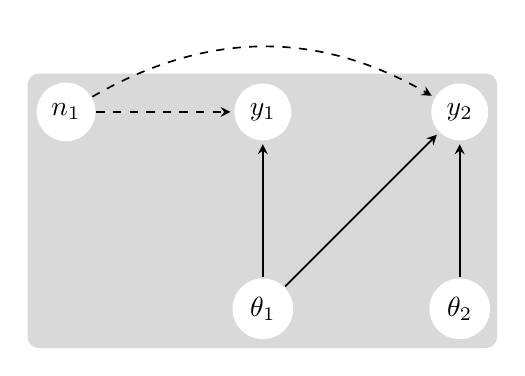
\begin{tikzpicture}[
            > = stealth, % arrow head style
            shorten > = 1pt, % don't touch arrow head to node
            auto,
            node distance = 2.5cm, % distance between nodes
            semithick % line style
        ]

        \tikzstyle{every state}=[
            draw = none,
            thick,
            fill = white,
            minimum size = 4mm
        ]F


	% data level
        \node[state] (Y) [] {$y_1$};
        \node[state] (N) [left of=Y] {$n_1$};
        \node[state] (Y2) [right of=Y] {$y_2$};
       
        \path[dashed,->] (N) edge node {} (Y);
        \path[dashed,->,bend left] (N) edge node {} (Y2);

         % parameters
         \node[state] (AB) [below of = Y] {$\theta_1$};
         \node[state] (AB2) [below of = Y2] {$\theta_2$};
                
         \path[->] (AB) edge node {} (Y);
         \path[->] (AB) edge node {} (Y2);
         \path[->] (AB2) edge node {} (Y2);
         
          \begin{scope}[on background layer]
   	  \node [fit=(N) (Y2) (AB), fill= gray!30, rounded corners, inner sep=.1cm] {};
          \end{scope}
          
  \end{tikzpicture}
  %
    \hspace{1cm}% NO SPACE!
  % BEGIN FIGURE 3
   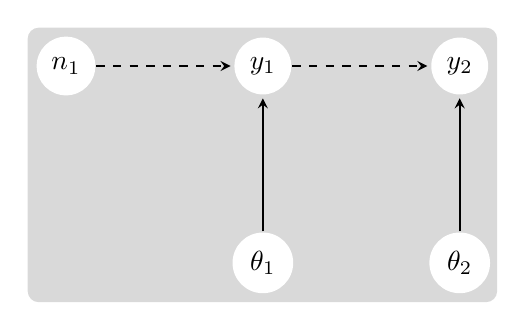
\begin{tikzpicture}[
              > = stealth, % arrow head style
            shorten > = 1pt, % don't touch arrow head to node
            auto,
            node distance = 2.5cm, % distance between nodes
            semithick % line style
        ]

        \tikzstyle{every state}=[
            draw = none,
            thick,
            fill = white,
            minimum size = 4mm
        ]F


	% data level
        \node[state] (Y) [] {$y_1$};
        \node[state] (N) [left of=Y] {$n_1$};
         \node[state] (Y2) [right of=Y] {$y_2$};
       
        \path[dashed,->] (N) edge node {} (Y);
        \path[dashed,->] (Y) edge node {} (Y2);

         % parameters
         \node[state] (AB) [below of = Y] {$\theta_1$};
         \node[state] (AB2) [below of = Y2] {$\theta_2$};
                
         \path[->] (AB) edge node {} (Y);
         \path[->] (AB2) edge node {} (Y2);
         
          \begin{scope}[on background layer]
   	  \node [fit=(N) (Y2) (AB), fill= gray!30, rounded corners, inner sep=.1cm] {};
          \end{scope}
                           
  \end{tikzpicture}
  %
\subcaption{Directed acyclic graphs for the hierarchical models for seed bag rates. Solid arrows depict the relationships among random variables, and dashed arrows depict the deterministic relationships.}
\end{subfigure}
\end{figure}
%
%%%%%%%%%%%%%%%%%%%%%%%%%%%%%%%%%%%%%%%%%%%%%%%%%%%%
% POSTERIOR AND JOINT DISTRIBUTIONS FOR AGE 1 SEED BAGS
%%%%%%%%%%%%%%%%%%%%%%%%%%%%%%%%%%%%%%%%%%%%%%%%%%%%

% QUESTIONS
% do I need to include \bm{n} on the RHS of the conditional statement for the posterior?

\begin{align}
  \begin{split}
 [  \theta_1, \theta_2  | & \bm{y_1} , \bm{y_2} ] \propto 
   \mathrm{binomial} ( y_1 | n_1, \mathrm{logit}^{-1}( \alpha_1 ) )  
      \\ & \times \mathrm{binomial} ( y_2 | n_1, \mathrm{logit}^{-1}( \alpha_1 ) \times \mathrm{logit}^{-1}( \alpha_2 ) ) 
   \\ & \times \mathrm{normal} ( \alpha_1  | \mu_1, \sigma_1 ) \mathrm{normal} ( \alpha_2  | \mu_2, \sigma_2 )
  \\ & \times \mathrm{normal} ( \mu_1 | 0 , 1000 ) \textrm{half-normal} ( \sigma_1 | 0,1)
    \\ & \times \mathrm{normal} ( \mu_2 | 0 , 1000 ) \textrm{half-normal} ( \sigma_2 | 0,1).
  \end{split}
\end{align}
%
\begin{align}
  \begin{split}
 [  \theta_1, \theta_2  | & \bm{y_1} , \bm{y_2} ] \propto 
   \mathrm{binomial} ( y_1 | n_1, \mathrm{logit}^{-1}( \alpha_1 ) )
      \\ & \times  \mathrm{binomial} ( y_2 | y_1, \mathrm{logit}^{-1}( \alpha_2 ) ) 
   \\ & \times \mathrm{normal} ( \alpha_1  | \mu_1, \sigma_1 ) \mathrm{normal} ( \alpha_2  | \mu_2, \sigma_2 )
  \\ & \times \mathrm{normal} ( \mu_1 | 0 , 1000 ) \textrm{half-normal} ( \sigma_1 | 0,1)
    \\ & \times \mathrm{normal} ( \mu_2 | 0 , 1000 ) \textrm{half-normal} ( \sigma_2 | 0,1).
  \end{split}
\end{align}
%

\clearpage
\newpage


\subsection*{Identifiability across years}
%%%%%%%%%%%%%%%%%%%%%%%%%%%%%%%%%%%%%%%%%%%%%%%%%%%%
% DIRECTED ACYCLIC GRAPHS FOR AGE 1 SEED BAGS
%%%%%%%%%%%%%%%%%%%%%%%%%%%%%%%%%%%%%%%%%%%%%%%%%%%%
\begin{figure}[h]%
\begin{subfigure}[c]{\textwidth}
   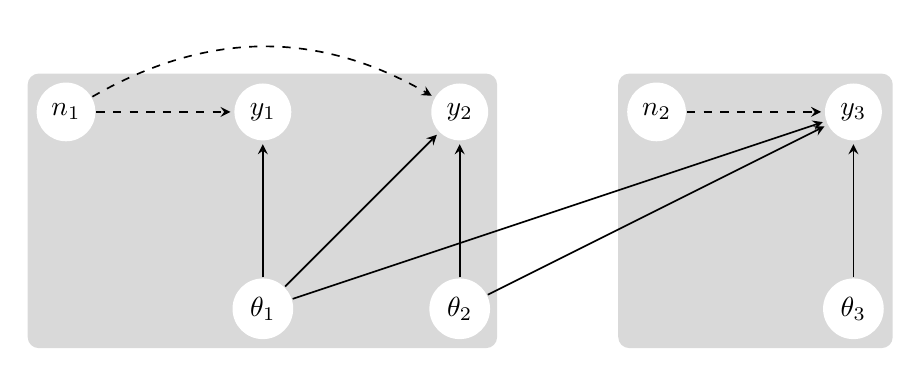
\begin{tikzpicture}[
            > = stealth, % arrow head style
            shorten > = 1pt, % don't touch arrow head to node
            auto,
            node distance = 2.5cm, % distance between nodes
            semithick % line style
        ]

        \tikzstyle{every state}=[
            draw = none,
            thick,
            fill = white,
            minimum size = 4mm
        ]F


	% data level
        \node[state] (Y) [] {$y_1$};
        \node[state] (N) [left of=Y] {$n_1$};
        \node[state] (Y2) [right of=Y] {$y_2$};
        \node[state] (N2) [right of=Y2] {$n_2$};
        \node[state] (Y3) [right of=N2] {$y_3$};
       
        \path[dashed,->] (N) edge node {} (Y);
        \path[dashed,->,bend left] (N) edge node {} (Y2);
        \path[dashed,->] (N2) edge node {} (Y3);

         % parameters
         \node[state] (AB) [below of = Y] {$\theta_1$};
         \node[state] (AB2) [below of = Y2] {$\theta_2$};
         \node[state] (AB3) [below of = Y3] {$\theta_3$};
                
         \path[->] (AB) edge node {} (Y);
         \path[->] (AB) edge node {} (Y2);
         \path[->] (AB2) edge node {} (Y2);
         \path[->] (AB) edge node {} (Y3);
         \path[->] (AB2) edge node {} (Y3);
         \path[->] (AB3) edge node {} (Y3);
         
          \begin{scope}[on background layer]
   	  \node [fit=(N) (Y2) (AB),fill=gray!30, rounded corners, inner sep=.1cm] {};
	  \node [fit=(N2) (Y3) (AB3),fill=gray!30, rounded corners, inner sep=.1cm] {};
          \end{scope}
          
  \end{tikzpicture} \\ \\ \\
   % BEGIN FIGURE 3
 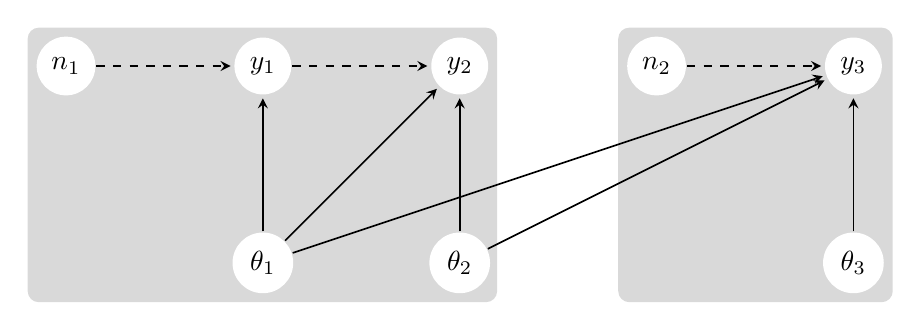
\begin{tikzpicture}[
            > = stealth, % arrow head style
            shorten > = 1pt, % don't touch arrow head to node
            auto,
            node distance = 2.5cm, % distance between nodes
            semithick % line style
        ]

        \tikzstyle{every state}=[
            draw = none,
            thick,
            fill = white,
            minimum size = 4mm
        ]F


	% data level
        \node[state] (Y) [] {$y_1$};
        \node[state] (N) [left of=Y] {$n_1$};
        \node[state] (Y2) [right of=Y] {$y_2$};
        \node[state] (N2) [right of=Y2] {$n_2$};
        \node[state] (Y3) [right of=N2] {$y_3$};
       
        \path[dashed,->] (N) edge node {} (Y);
        \path[dashed,->] (Y) edge node {} (Y2);
        \path[dashed,->] (N2) edge node {} (Y3);

         % parameters
         \node[state] (AB) [below of = Y] {$\theta_1$};
         \node[state] (AB2) [below of = Y2] {$\theta_2$};
         \node[state] (AB3) [below of = Y3] {$\theta_3$};
                
         \path[->] (AB) edge node {} (Y);
         \path[->] (AB) edge node {} (Y2);
         \path[->] (AB2) edge node {} (Y2);
         \path[->] (AB) edge node {} (Y3);
         \path[->] (AB2) edge node {} (Y3);
         \path[->] (AB3) edge node {} (Y3);
         
          \begin{scope}[on background layer]
   	  \node [fit=(N) (Y2) (AB),fill=gray!30, rounded corners, inner sep=.1cm] {};
	  \node [fit=(N2) (Y3) (AB3),fill=gray!30, rounded corners, inner sep=.1cm] {};
          \end{scope}
          
  \end{tikzpicture}
  %
\subcaption{Directed acyclic graphs for the hierarchical models for seed bag rates. Solid arrows depict the relationships among random variables, and dashed arrows depict the deterministic relationships.}
\end{subfigure}
\end{figure}
%
%%%%%%%%%%%%%%%%%%%%%%%%%%%%%%%%%%%%%%%%%%%%%%%%%%%%
% POSTERIOR AND JOINT DISTRIBUTIONS FOR AGE 1 SEED BAGS
%%%%%%%%%%%%%%%%%%%%%%%%%%%%%%%%%%%%%%%%%%%%%%%%%%%%

% QUESTIONS
% do I need to include \bm{n} on the RHS of the conditional statement for the posterior?

\begin{align}
  \begin{split}
 [  \theta_1, \theta_2  | & \bm{y_1} , \bm{y_2} ] \propto 
   \mathrm{binomial} ( y_1 | n_1, \mathrm{logit}^{-1}( \alpha_1 ) )  
      \\ & \times \mathrm{binomial} ( y_2 | n_1, \mathrm{logit}^{-1}( \alpha_1 ) \times \mathrm{logit}^{-1}( \alpha_2 ) ) 
   \\ & \times \mathrm{normal} ( \alpha_1  | \mu_1, \sigma_1 ) \mathrm{normal} ( \alpha_2  | \mu_2, \sigma_2 )
  \\ & \times \mathrm{normal} ( \mu_1 | 0 , 1000 ) \textrm{half-normal} ( \sigma_1 | 0,1)
    \\ & \times \mathrm{normal} ( \mu_2 | 0 , 1000 ) \textrm{half-normal} ( \sigma_2 | 0,1).
  \end{split}
\end{align}
%
\begin{align}
  \begin{split}
 [  \theta_1, \theta_2  | & \bm{y_1} , \bm{y_2} ] \propto 
   \mathrm{binomial} ( y_1 | n_1, \mathrm{logit}^{-1}( \alpha_1 ) )
      \\ & \times  \mathrm{binomial} ( y_2 | y_1, \mathrm{logit}^{-1}( \alpha_2 ) ) 
   \\ & \times \mathrm{normal} ( \alpha_1  | \mu_1, \sigma_1 ) \mathrm{normal} ( \alpha_2  | \mu_2, \sigma_2 )
  \\ & \times \mathrm{normal} ( \mu_1 | 0 , 1000 ) \textrm{half-normal} ( \sigma_1 | 0,1)
    \\ & \times \mathrm{normal} ( \mu_2 | 0 , 1000 ) \textrm{half-normal} ( \sigma_2 | 0,1).
  \end{split}
\end{align}
%

\clearpage
\newpage

\subsection*{Exponential decay}
%%%%%%%%%%%%%%%%%%%%%%%%%%%%%%%%%%%%%%%%%%%%%%%%%%%%
% DIRECTED ACYCLIC GRAPHS FOR AGE 1 SEED BAGS
%%%%%%%%%%%%%%%%%%%%%%%%%%%%%%%%%%%%%%%%%%%%%%%%%%%%
\begin{figure}[h]%
\begin{subfigure}[c]{\textwidth}
   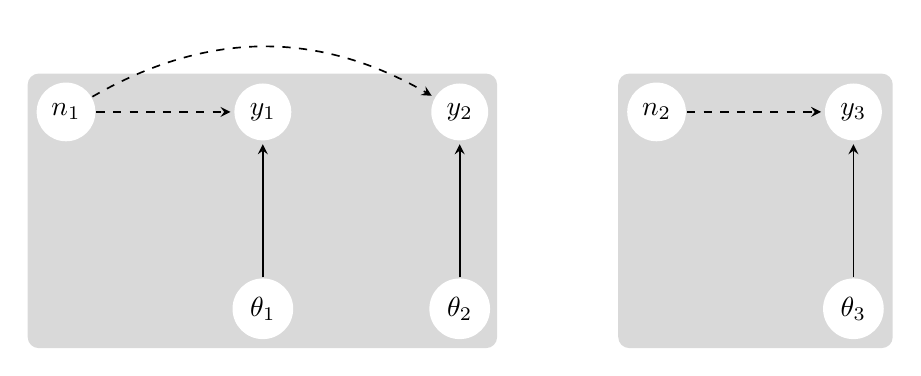
\begin{tikzpicture}[
            > = stealth, % arrow head style
            shorten > = 1pt, % don't touch arrow head to node
            auto,
            node distance = 2.5cm, % distance between nodes
            semithick % line style
        ]

        \tikzstyle{every state}=[
            draw = none,
            thick,
            fill = white,
            minimum size = 4mm
        ]F


	% data level
        \node[state] (Y) [] {$y_1$};
        \node[state] (N) [left of=Y] {$n_1$};
        \node[state] (Y2) [right of=Y] {$y_2$};
        \node[state] (N2) [right of=Y2] {$n_2$};
        \node[state] (Y3) [right of=N2] {$y_3$};
       
        \path[dashed,->] (N) edge node {} (Y);
        \path[dashed,->,bend left] (N) edge node {} (Y2);
        \path[dashed,->] (N2) edge node {} (Y3);

         % parameters
         \node[state] (AB) [below of = Y] {$\theta_1$};
         \node[state] (AB2) [below of = Y2] {$\theta_2$};
         \node[state] (AB3) [below of = Y3] {$\theta_3$};
                
         \path[->] (AB) edge node {} (Y);
         \path[->] (AB2) edge node {} (Y2);
         \path[->] (AB3) edge node {} (Y3);
         
          \begin{scope}[on background layer]
   	  \node [fit=(N) (Y2) (AB),fill=gray!30, rounded corners, inner sep=.1cm] {};
	  \node [fit=(N2) (Y3) (AB3),fill=gray!30, rounded corners, inner sep=.1cm] {};
          \end{scope}
          
  \end{tikzpicture} \\ \\ \\
   % BEGIN FIGURE 3
 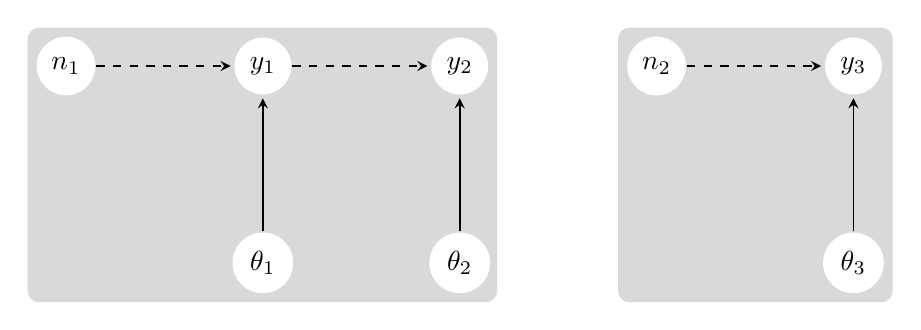
\begin{tikzpicture}[
            > = stealth, % arrow head style
            shorten > = 1pt, % don't touch arrow head to node
            auto,
            node distance = 2.5cm, % distance between nodes
            semithick % line style
        ]

        \tikzstyle{every state}=[
            draw = none,
            thick,
            fill = white,
            minimum size = 4mm
        ]F


	% data level
        \node[state] (Y) [] {$y_1$};
        \node[state] (N) [left of=Y] {$n_1$};
        \node[state] (Y2) [right of=Y] {$y_2$};
        \node[state] (N2) [right of=Y2] {$n_2$};
        \node[state] (Y3) [right of=N2] {$y_3$};
       
        \path[dashed,->] (N) edge node {} (Y);
        \path[dashed,->] (Y) edge node {} (Y2);
        \path[dashed,->] (N2) edge node {} (Y3);

         % parameters
         \node[state] (AB) [below of = Y] {$\theta_1$};
         \node[state] (AB2) [below of = Y2] {$\theta_2$};
         \node[state] (AB3) [below of = Y3] {$\theta_3$};
                
         \path[->] (AB) edge node {} (Y);
         \path[->] (AB2) edge node {} (Y2);
         \path[->] (AB3) edge node {} (Y3);
         
          \begin{scope}[on background layer]
   	  \node [fit=(N) (Y2) (AB),fill=gray!30, rounded corners, inner sep=.1cm] {};
	  \node [fit=(N2) (Y3) (AB3),fill=gray!30, rounded corners, inner sep=.1cm] {};
          \end{scope}
          
  \end{tikzpicture}
  %
\subcaption{Directed acyclic graphs for the hierarchical models for seed bag rates. Solid arrows depict the relationships among random variables, and dashed arrows depict the deterministic relationships.}
\end{subfigure}
\end{figure}

\end{document}
